% Generated by Sphinx.
\def\sphinxdocclass[english]{xmosmodern}
\documentclass[  document]{xmosmodern}
\usepackage[utf8]{inputenc}
\DeclareUnicodeCharacter{00A0}{\nobreakspace}

\usepackage{longtable}



\title{Display Controller Demo Quickstart Guide}
\date{November 15, 2013}
\author{}
\newcommand{\sphinxlogo}{}
\newcommand{\releasename}{Release}
\usepackage{xsphinx}
\usepackage{threeparttable}
\usepackage{fancyvrb}
\usepackage{indent}
\renewcommand\bfcode\textbf
\renewcommand\bf\textbf
\graphicspath{{./}{./images/}}
\makeindex

\newcommand\PYGZat{@}
\newcommand\PYGZlb{[}
\newcommand\PYGZrb{]}

\setlength{\emergencystretch}{8em}
\start

\maketitle
\pretoc
\phantomsection\label{quickstart::doc}

%last summary
\begin{inthisdocument}
\item \nameref{quickstart:sw-display-controller-demo-quick-start-guide}
\end{inthisdocument}


% NON-FULLWIDTH SECTION



% NON-FULLWIDTH SECTION
\section{sw\_display\_controller demo : Quick Start Guide}
\label{quickstart:sw-display-controller-demo-quick-start-guide}\label{quickstart:display-controller-demo-quickstart}\label{quickstart:display-controller-demo-quickstart-guide}\begin{description}
\item[In this demonstration we use the following hardware and software:]\begin{itemize}
\item   XP-SKC-L16 sliceKIT

\item   XA-SK-SCR480 Slice Card,

\item   XA-SK-SDRAM Slice Card,

\item   module\_sdram,

\item   module\_lcd,

\item   module\_display\_controller,

\item   module\_i2c\_master,

\item   module\_touch\_controller\_lib,

\item   module\_slicekit\_support,

\end{itemize}


\end{description}



together to create an interactive display on LCD. This application showcases some of the key software
features and serves as an example on how to use an LCD without the real-time constraint of having to
update the LCD line buffer and how to use the touch screen for interactive display.



% NON-FULLWIDTH SECTION
\subsection{Hardware Setup}
\label{quickstart:hardware-setup}

The XP-SKC-L16 sliceKIT Core board has four slots with edge connectors: \verb`SQUARE`, \verb`CIRCLE`, \verb`TRIANGLE`
and \verb`STAR`.


To setup up the system:
\begin{enumerate}
\item   Connect XA-SK-SDRAM Slice Card to the XP-SKC-L16 sliceKIT Core board using the connector marked with the \verb`STAR`.

\item   Connect XA-SK-SCR480 Slice Card to the XP-SKC-L16 sliceKIT Core board using the connector marked with the \verb`TRIANGLE`.

\item   Connect the xTAG Adapter to sliceKIT Core board, and connect xTAG-2 to the adapter.

\item   Connect the xTAG-2 to host PC. Note that the USB cable is not provided with the sliceKIT starter kit.

\item   Set the \verb`xCONNECT LINK` to \verb`OFF` on the xTAG Adapter(XA-SK-XTAG2).

\item   Ensure the jumper on the XA-SK-SCR480 is bridged if the back light is required.

\item   Switch on the power supply to the sliceKIT Core board.

\end{enumerate}

\begin{figure}[h]
\begin{sidecaption}{Hardware Setup for Display Controller Demo}

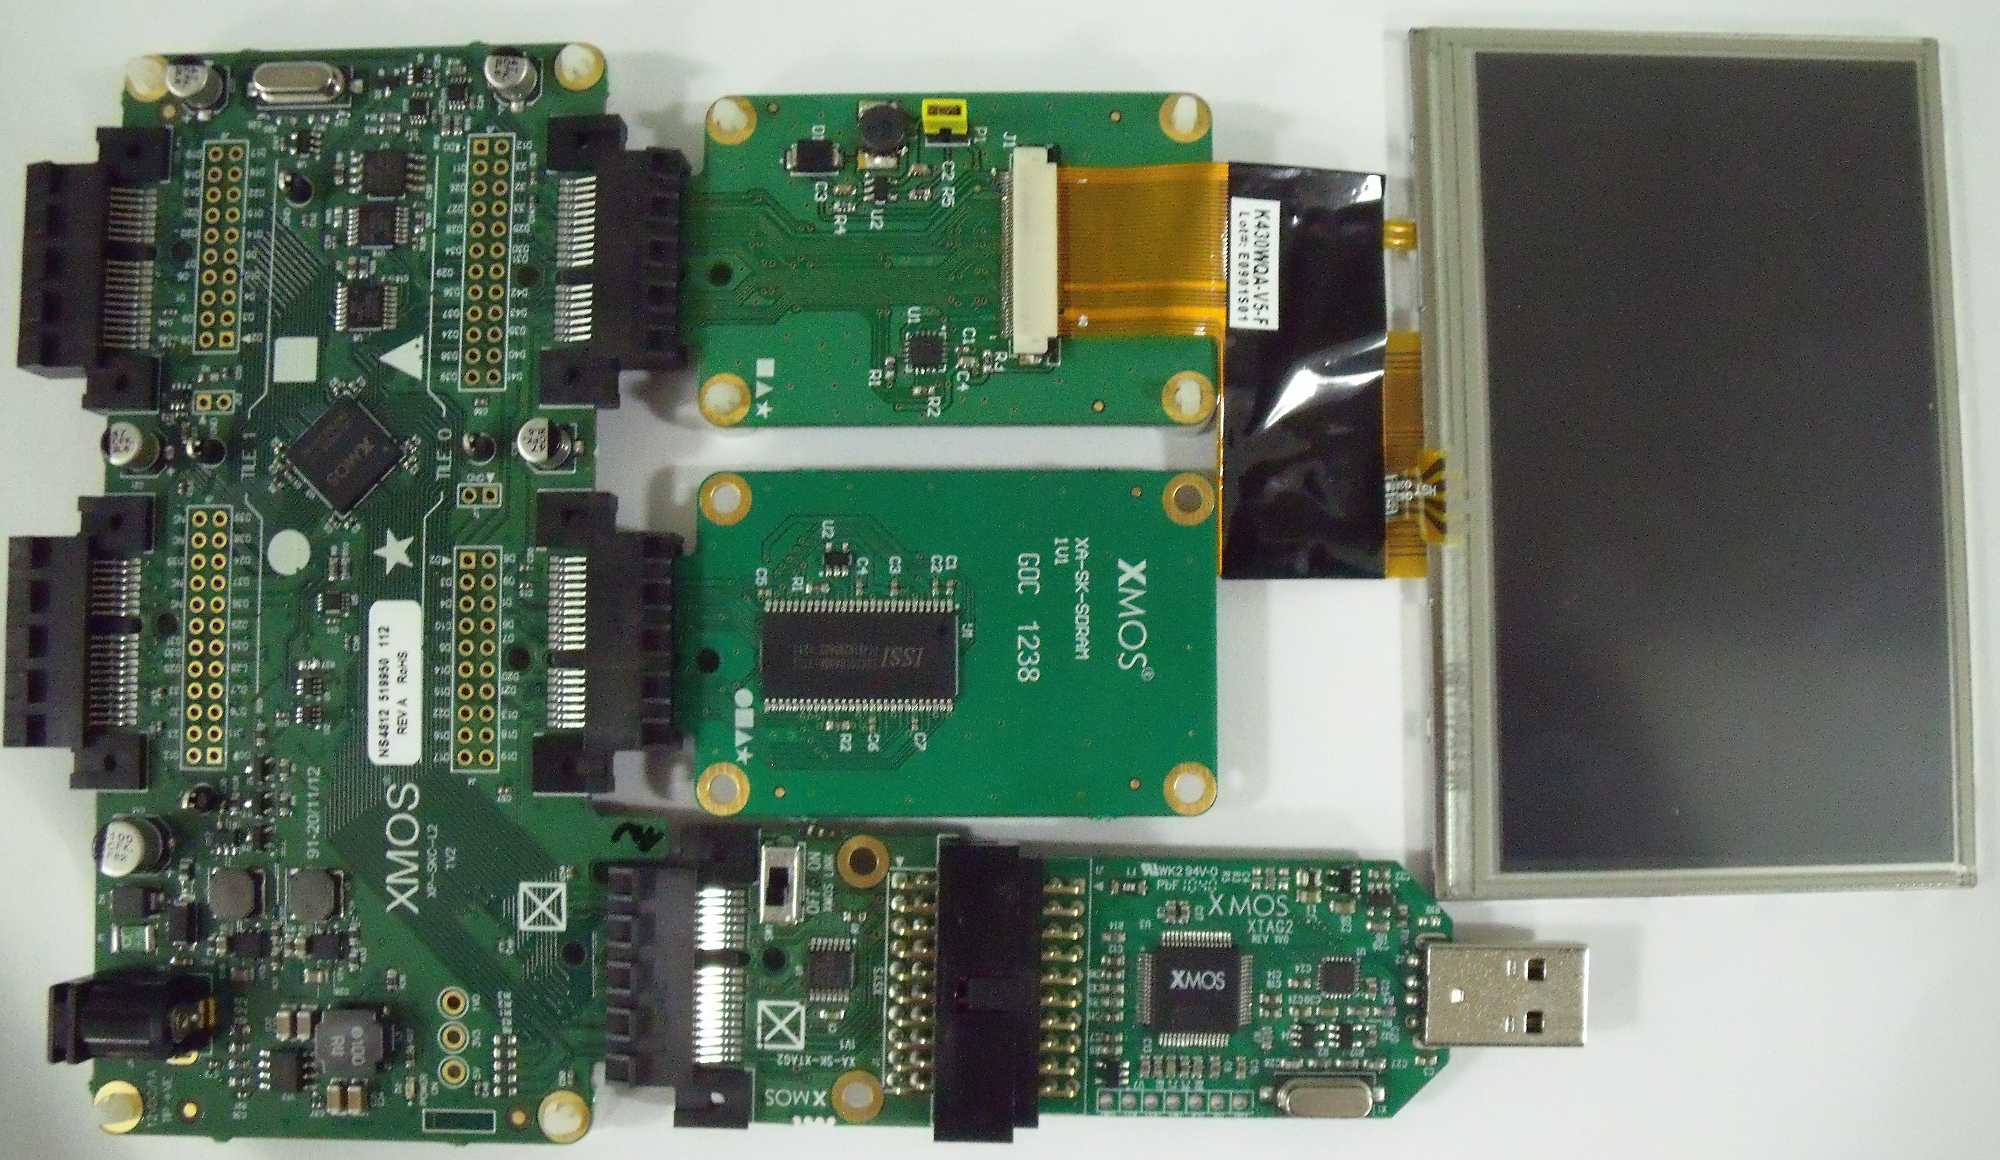
\includegraphics{hardware_setup.jpg}
\end{sidecaption}\end{figure} \DocumentFooterFix



% NON-FULLWIDTH SECTION
\subsection{Import and Build the Application}
\label{quickstart:import-and-build-the-application}\begin{enumerate}
\item   Open xTIMEcomposer and check that it is operating in online mode. Open the edit perspective (Window-\textgreater{}Open Perspective-\textgreater{}XMOS Edit).

\item   Locate the \verb`'Display Controller Demo'` item in the xSOFTip pane on the bottom left of the window and drag it into the Project Explorer window in the xTIMEcomposer. This will also cause the modules on which this application depends to be imported as well.

\item   Click on the app\_display\_controller\_demo item in the Explorer pane then click on the build icon (hammer) in xTIMEcomposer. Check the console window to verify that the application has built successfully.

\item   There will be quite a number of warnings that \verb`bidirectional buffered port not supported in hardware`. These can be safely ignored for this component.

\end{enumerate}



For help in using xTIMEcomposer, try the xTIMEcomposer tutorial, which you can find by selecting Help-\textgreater{}Tutorials from the xTIMEcomposer menu.


Note that the Developer Column in the xTIMEcomposer on the right hand side of your screen provides information on the xSOFTip components you are using. Select the module\_display\_controller component in the Project Explorer, and you will see its description together with API documentation. Having done this, click the \emph{back} icon until you return to this quickstart guide within the Developer Column.



% NON-FULLWIDTH SECTION
\subsection{Run the Application}
\label{quickstart:run-the-application}

Now that the application has been compiled, the next step is to run it on the sliceKIT Core Board using the tools to load the application over JTAG (via the xTAG-2 and xTAG Adapter card) into the xCORE multicore microcontroller.
\begin{enumerate}
\item   Select the file \verb`app_display_controller_demo.xc` in the \verb`app_display_controller_demo` project from the Project Explorer.

\item   Click on the \verb`Run` icon (the white arrow in the green circle).

\item   At the \verb`Select Device` dialog select \verb`XMOS xTAG-2 connect to L1[0..1]` and click \verb`OK`.

\item   Wait until the images have loaded over the xTAG connector from the host, this should take approximately 21 seconds.

\item   There should be a series of 6 images for transition from one to another.

\item   Once the first image is displayed, a message is displayed on the console to prompt the user to touch any of the corners or the center of LCD screen for watching different transition effects.

\end{enumerate}




% NON-FULLWIDTH SECTION
\subsection{Next Steps}
\label{quickstart:next-steps}\begin{enumerate}
\item   Try changing the files that are loaded from the host. To do this, generate an image of 480 by 272 pixels, save it in \verb`tga` format uncompressed in ``top left'' format (``bottom left'' will also work but the image will have to be upside-down). Save the file(s) into \verb`the app_display_controller_demo` directory within your workspace. Now, increment the \verb`IMAGE_COUNT` define to 7 and add the name of your new image to the array \verb`images`. Ensure the filename is less than 30 characters long.

\item   Each transition has a frame count that configures the speed of the transition, try adjusting them and observe the results. To do this take a look at the API for the display controller. Note how each of the transition effects have a \verb`frame_count` parameter. This parameter specifies how many frames the transition should take.

\item   Try writing an exciting transition effect. To do this, begin with the template shown below and refer to the Display Controller API documentation.

\vspace{-5pt}\begin{minipage}{\linewidth}
\begin{lstlisting}[basicstyle=\ttfamily\Smaller]
static void transition_exciting_impl(chanend server, unsigned next_image_fb,
   unsigned image_from, unsigned image_to, unsigned line) {
   //insert code here
}
unsigned transition_exciting(chanend server, unsigned frame_buf[2],
  unsigned from, unsigned to, unsigned frames, unsigned cur_fb_index) {
  unsigned next_fb_index;
  for (unsigned frame = 0; frame < frames; frame++) {
    next_fb_index = (cur_fb_index + 1) & 1;
    for (unsigned line = 0; line < LCD_HEIGHT; line++)
      transition_exciting_impl(server, frame_buf[next_fb_index], from, to, line);
    frame_buffer_commit(server, frame_buf[next_fb_index]);
    cur_fb_index = next_fb_index;
  }
  return cur_fb_index;
}
\end{lstlisting}
\end{minipage}


\end{enumerate}





\finish
